\documentclass[slidestop,compress,mathserif,xcolor=svgnames,table,xcolor=dvipsnames]{beamer}

\usepackage[spanish]{babel}
\usepackage[utf8]{inputenc} % Ambos para solucin de asuntos de idioma.
\usepackage{amsmath, amsfonts, amssymb} % Matemticas varias.
\usepackage{longtable} % Tabla larga necesaria para el apndice de simbologa.
%\usepackage{multimedia}
\usepackage{movie15}
\usepackage{enumitem}
\usepackage{lmodern}
\usepackage{tikz}

\setitemize{leftmargin=*}
\setitemize[1]{label=\tiny$\blacksquare$}
\setitemize[2]{label=\tiny$\bullet$}
\setitemize[3]{label=\tiny$\bullet$}
% \setbeamertemplate{sections in toc}[ball]

% --- Arreglos varios para la inclusion de imgenes
\usepackage{subfigure}
\DeclareGraphicsExtensions{.png,.jpg,.pdf,.mps,.gif,.bmp}

% ================= CONFIGURACIN DEL BEAMER ====================
% ===============================================================
\mode<presentation>{
% \usepackage{beamerthemeclassic}
% \setbeameroption{show notes}
% \setbeameroption{hide notes}
\setbeameroption{notes on second screen}
% \setbeamercovered{transparent}

% \usetheme{Warsaw}
% \usetheme{Frankfurt}
% \usetheme{Berlin}
% \usetheme{Madrid}
% \usetheme{Antibes}
% \usetheme{Darmstadt}
% \usetheme{Marburg}
% \usetheme{CambridgeUS}
% \usetheme{PaloAlto}
% \usetheme{AnnArbor}
\usetheme{Warsaw}
% \usecolortheme{rose}
% \usecolortheme{lily}
% \usecolortheme{seahorse}
% \usecolortheme{fly}
% \usecolortheme[RGB={70,110,45}]{structure}	% verde primaveral
% \usecolortheme[RGB={100,12,20}]{structure}	% rojo sangre
% \usecolortheme[RGB={30,40,30}]{structure}	    % Luto
% \usecolortheme[RGB={160,230,70}]{structure}	% verde manzana Grand-Smith

% \beamertemplateshadingbackground{green!30}{white}

% \usefonttheme[onlymath]{serif}
% \usefonttheme{professionalfonts}
\usefonttheme{structurebold}

% \setbeamerfont{frametitle}{family=\rmfamily,shape=\scshape,size=\normalsize}
% \setbeamertemplate{frametitle}[default][center]
% \setbeamerfont{section number projected}{family=\rmfamily,series=\bfseries,size=\tiny}
\setbeamercolor{section number projected}{bg=white,fg=black}


}
% Make a TOC appear before every section
%\AtBeginSection[]{
%\begin{frame}
%	\tableofcontents[currentsection]
%\end{frame}
%}

\AtBeginNote{Notas:\par}


% ========================= COMANDOS ============================
% ===============================================================
\newcommand{\ket}[1]{|#1\rangle}
\newcommand{\bcol}{\begin{columns}[T]}
\newcommand{\ecol}{\end{columns}}
\newcommand{\col}[1][0.5]{\column{#1\textwidth}}
\newenvironment{itemize*}%
  {\begin{itemize}%
    \setlength{\topsep}{10pt}%
    \setlength{\itemsep}{0pt}%
    \setlength{\parskip}{10pt}}%
  {\end{itemize}
}

% =================== DATOS DEL DOCUMENTO =======================
% ===============================================================
\author{Gonzalo Gutiérrez, Matias Tailanián}
\date{19 de Octubre de 2012}
\title{\textit{Seguimiento de Tempo}}
\subtitle{Procesamiento digital de señales de audio\\Curso 2012}



% ===============================================================
% ===============================================================
% ================ COMIENZO DEL DOCUMENTO =======================
% ===============================================================
% ===============================================================



\begin{document}

% ========================= FRAME ===============================
% ===============================================================
\begin{frame}
  \titlepage
\end{frame}


\section{Gral}
% ========================= FRAME ===============================
% ===============================================================
\begin{frame}
\frametitle{IBT: Real tempo and Beat-Tracking system}

\begin{columns}

\column{2in}
\vspace{15pt}
\begin{figure}[h!]
  \begin{center}
  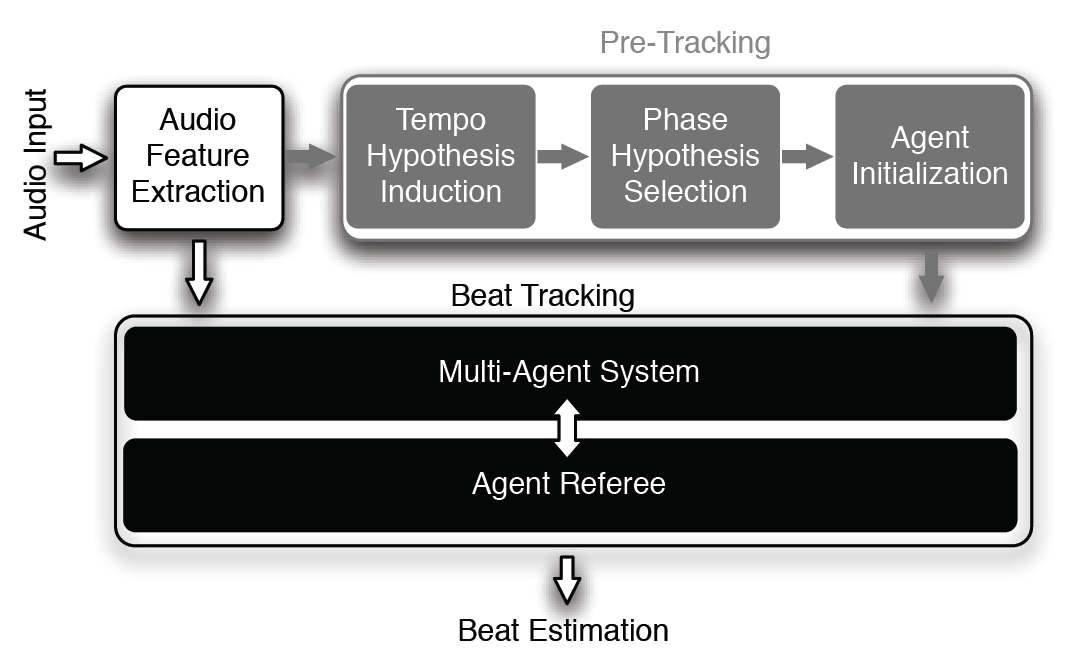
\includegraphics[width=1\textwidth]{./pics/bloques.png}
  \end{center}
  \vspace{-10pt}
  \caption{Diagrama de bloques}
  \label{fig:bloques}
\end{figure}

\column{2in}
\vspace{20pt}
\begin{itemize}
	\item \textbf{Feature Selection}\pause
	\item \textbf{Pre Tracking}\\\pause
  	\begin{itemize*}
	  \item Período
	  \item Fase
	  \item Agente\pause
	\end{itemize*}
	\item \textbf{Beat tracking}\pause
    \item \textbf{Ejemplos}
    \item \textbf{Conclusiones}
\end{itemize}

\end{columns}
\end{frame}


\section{Feature Selection}
% ========================= FRAME ===============================
% ===============================================================
\begin{frame}
\frametitle{Feature Selection}
\begin{columns}

% -----------------------------------------------------------------
\column{1.5in}
\vspace*{15pt}
\begin{scriptsize}
	\begin{itemize} \item \textbf{Onset detection} \end{itemize}
\begin{scriptsize}
    \uncover<2->{
	\begin{equation*}
		SF(n) = \sum\limits_{k=-\frac{\omega}{2}}^{\frac{\omega}{2}-1}\color<3->{red}HWR(\color<3->{black}|X(n,k)|-|X(n-1,k)|\color<3->{red})\color<3->{black}
		\label{ec:autocorrelacion}
	\end{equation*}
    }
\end{scriptsize}

\uncover<3->{
	\color<3->{red}$HWR(x)=\frac{x+|x|}{2}$\color<3->{black} es la rectificación de media onda de $x$, solo nos interesa las variaciones
    crecientes en el espectro.
}

\end{scriptsize}
% -----------------------------------------------------------------

% -----------------------------------------------------------------
\column{3in}
\vspace*{15pt}
\begin{scriptsize}


\only<1->{
\vspace*{25pt}
%\begin{figure}
\begin{center}
\begin{tikzpicture}
\alt<2->
{\node[opacity=1]
{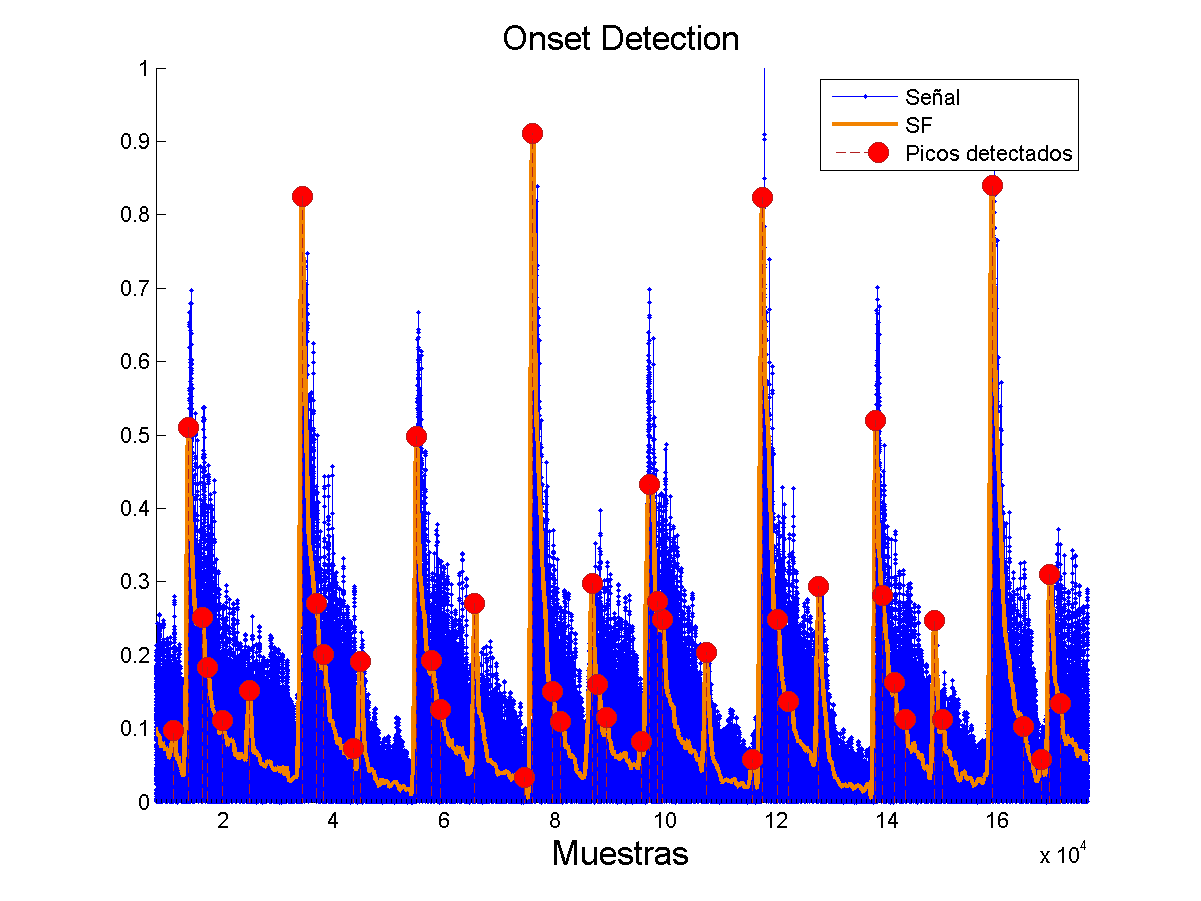
\includegraphics[width=0.9\textwidth]{./pics/SF.png}};}
{\node[opacity=.15]
{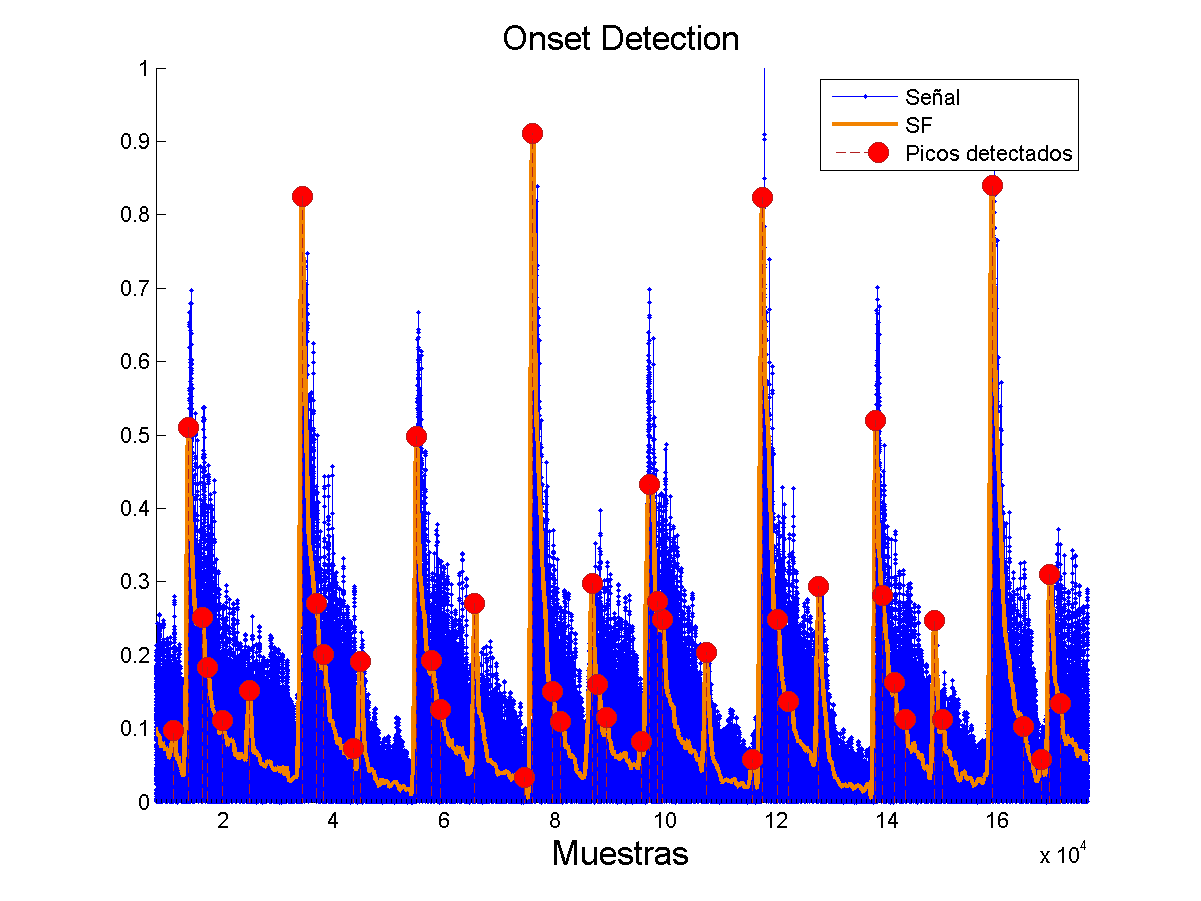
\includegraphics[width=0.9\textwidth]{./pics/SF.png}};}
\end{tikzpicture}
\end{center}
%\end{figure}
}



\end{scriptsize}
% -----------------------------------------------------------------


\end{columns}
\end{frame}







\section{Pre-Tracking}
% ========================= FRAME ===============================
% ===============================================================
\begin{frame}
\frametitle{Pre-Tracking}
\begin{columns}

% -----------------------------------------------------------------
\column{1.5in}
\vspace*{15pt}
\begin{scriptsize}

\only<1,2,3,4,5,6>{
    \begin{itemize} \item<1-> \textbf{Período} \end{itemize}

    \visible<2->{
    \alert<3>{
	\begin{equation*}
		A(\tau) = \sum\limits_{n=0}^{m}SF(n)SF(n+\tau)
		\label{ec:autocorrelacion}
	\end{equation*}
    }
	
    $SF$ es el flujo espectral suavizado para el \emph{frame} $n$
	 }
    \uncover<4,5,6>{
    \alert<6>{
    \begin{equation*}
		\begin{cases}
		P_i = \arg\max_i \left\{ A(\tau) \right\}, & i=1,\dots, N\\
		A(\tau)>\delta \frac{rms(A(\tau))}{M} &
		\end{cases}
		\label{ec:period}
	\end{equation*}
    }
    $\delta$ es un umbral determinado empíricamente y $M$ es un rango de tiempos definido entre [50,250] BPM.
    }
    }
\only<7-17>{
\begin{itemize} \item \textbf{Fase} \end{itemize}
\only<8,9,10,11>{
\uncover<8,9,10,11>{
Para cada \alert<9>{$P_i$} estimado se generan j hipótesis de fase: \alert<10>{$\phi_i^j$}. Se supone fase y períodos constantes en cada ventana de análisis.\\

Se utiliza un \alert<11>{\emph{template} de tren de pulsos} para ver cuál ajusta mejor.\\[.5cm]
}
}
}
\only<12-17>{
\begin{description}
  \item {\textbf{-Mejor fase:}
  \only<13->{
  Se obtiene cuando al ``mover'' el tren de pulsos se alcanza un máximo en el puntaje que arroja la siguiente ecuación:
}
}
\end{description}

\only<14->{
\begin{equation*}
S_i=\color<15->{red}{{S_i}^{rel}}\color<15->{black}*max(\color<17->{blue}{S_i}^{raw}\color<17->{black})
\end{equation*}

\only<15-17>{
donde:
\begin{equation*}
\color<15->{red}{S_i}^{rel}\color<15->{black}=10*\color<17->{blue}{S_i}^{raw}\color<17->{black}+ \sum\limits_{j=0}^{N}\color<16->{green}r(n_{ij})\color<16->{black}*\color<17->{blue}{S_j}^{raw}\color<17->{black}
		\label{ec:autocorrelacion}
\end{equation*}
}

}

}

\only<18->{
\begin{itemize} \item \textbf{Agentes} \end{itemize}
\only<19->{
Las hipótesis estimadas $(P_i,\phi_i,S_i)$ pueden ser ahora utilizadas para inicializar un conjunto de N
agentes en el cual cada uno empezará a realizar su propio beat tracking
}
}
\end{scriptsize}

% -----------------------------------------------------------------


% -----------------------------------------------------------------
\column{3in}
\vspace*{15pt}

\begin{scriptsize}

\only<1,2,3,4,5>{
\begin{tikzpicture}
\alt<3->
{\node[opacity=1]
{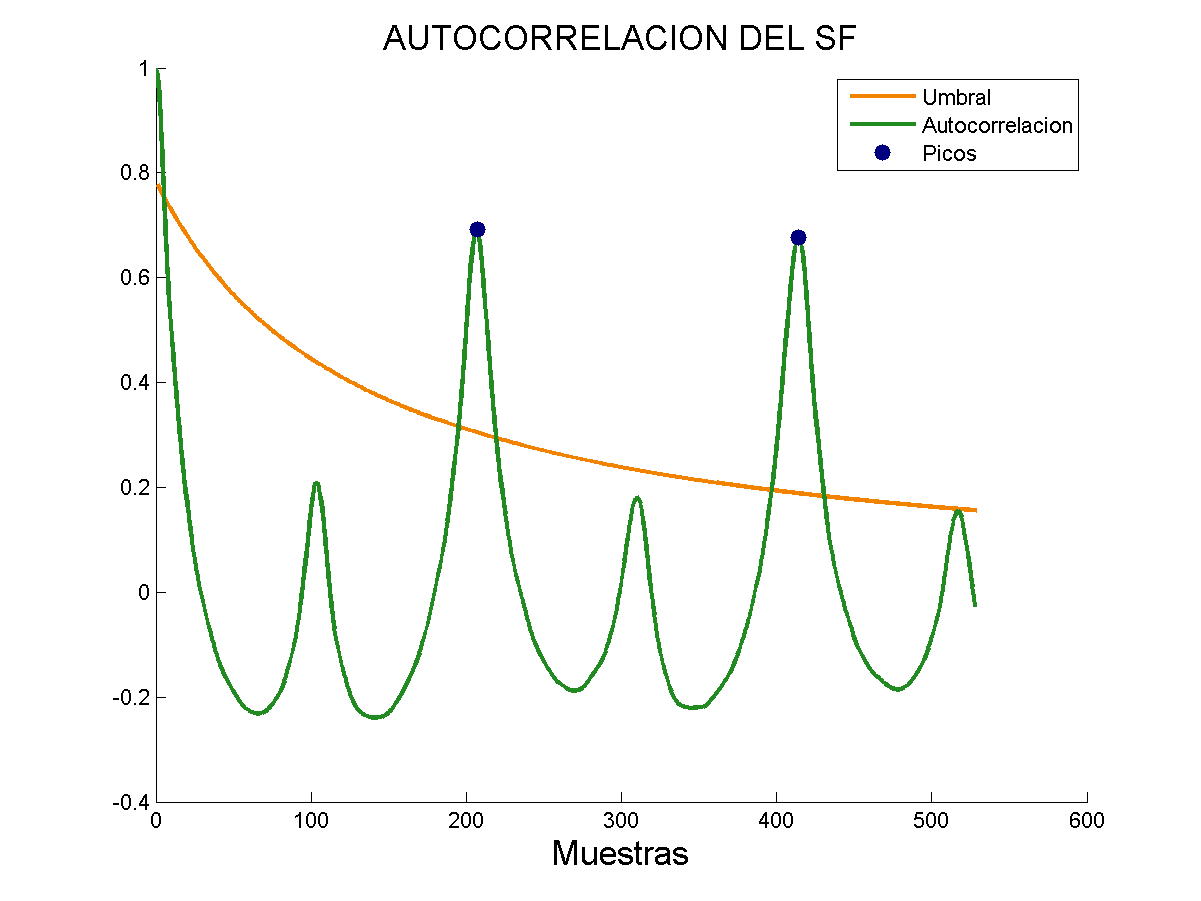
\includegraphics[width=1\textwidth]{./pics/ACF.png}};}
{\node[opacity=.15]
{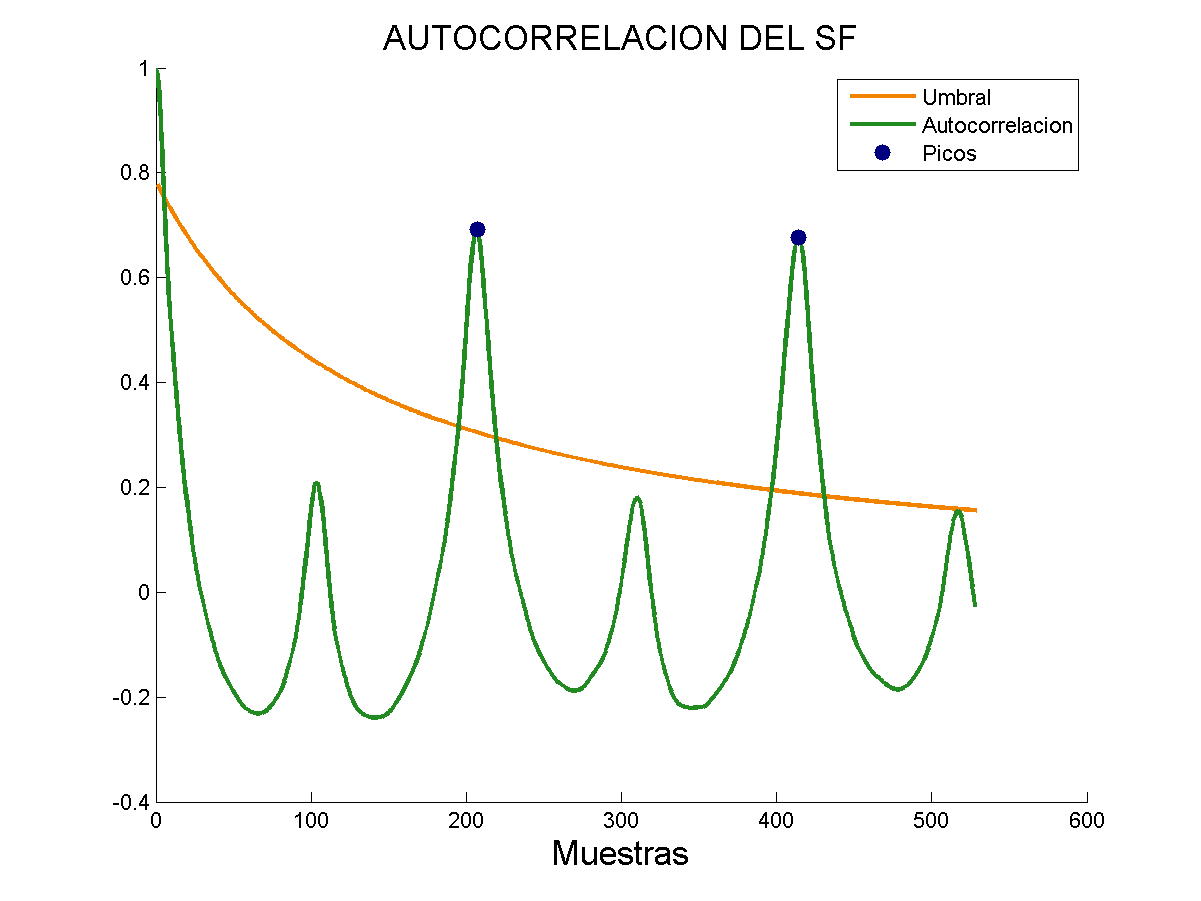
\includegraphics[width=1\textwidth]{./pics/ACF.png}};}
\end{tikzpicture}
}

\only<6>{
\begin{tikzpicture}
\alt<6->
{\node[opacity=1]
{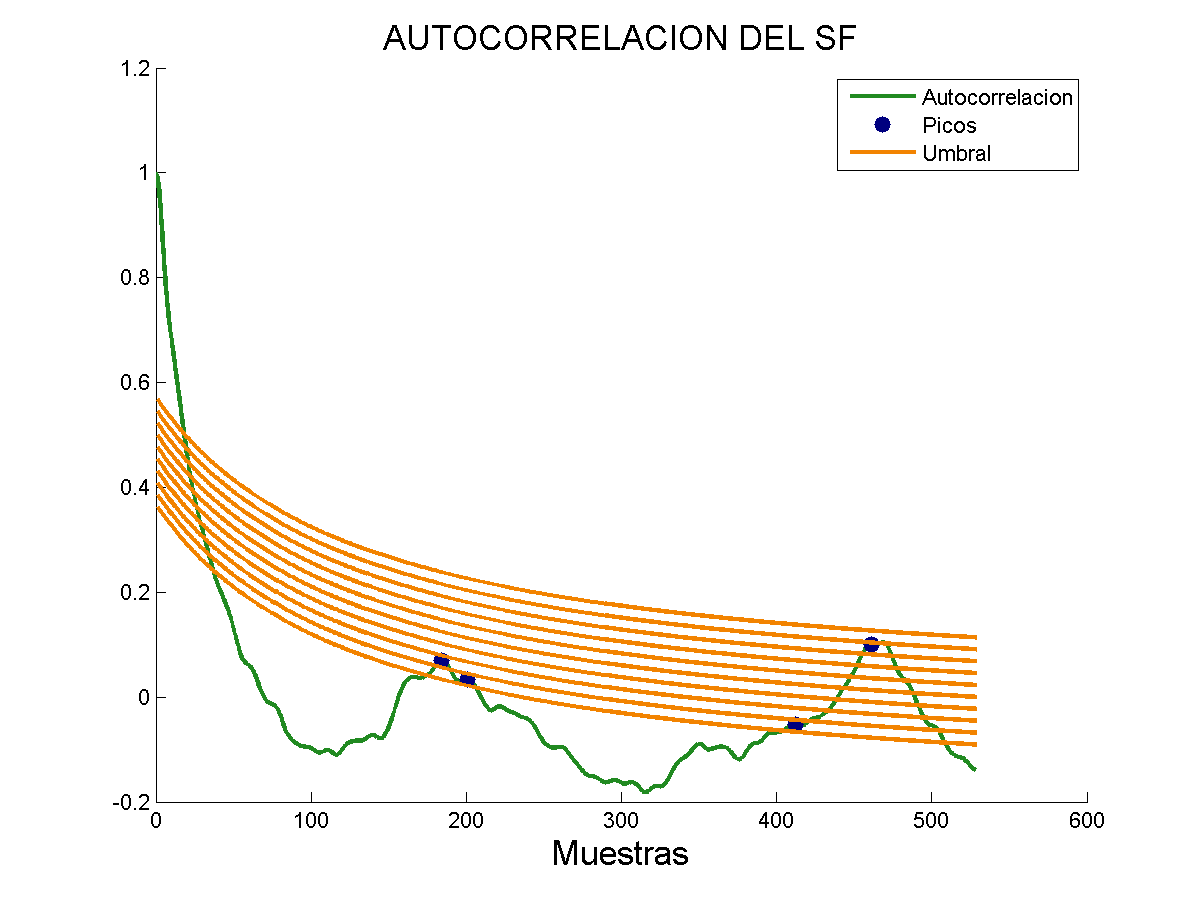
\includegraphics[width=1\textwidth]{./pics/ACF2.png}};}
{\node[opacity=.15]
{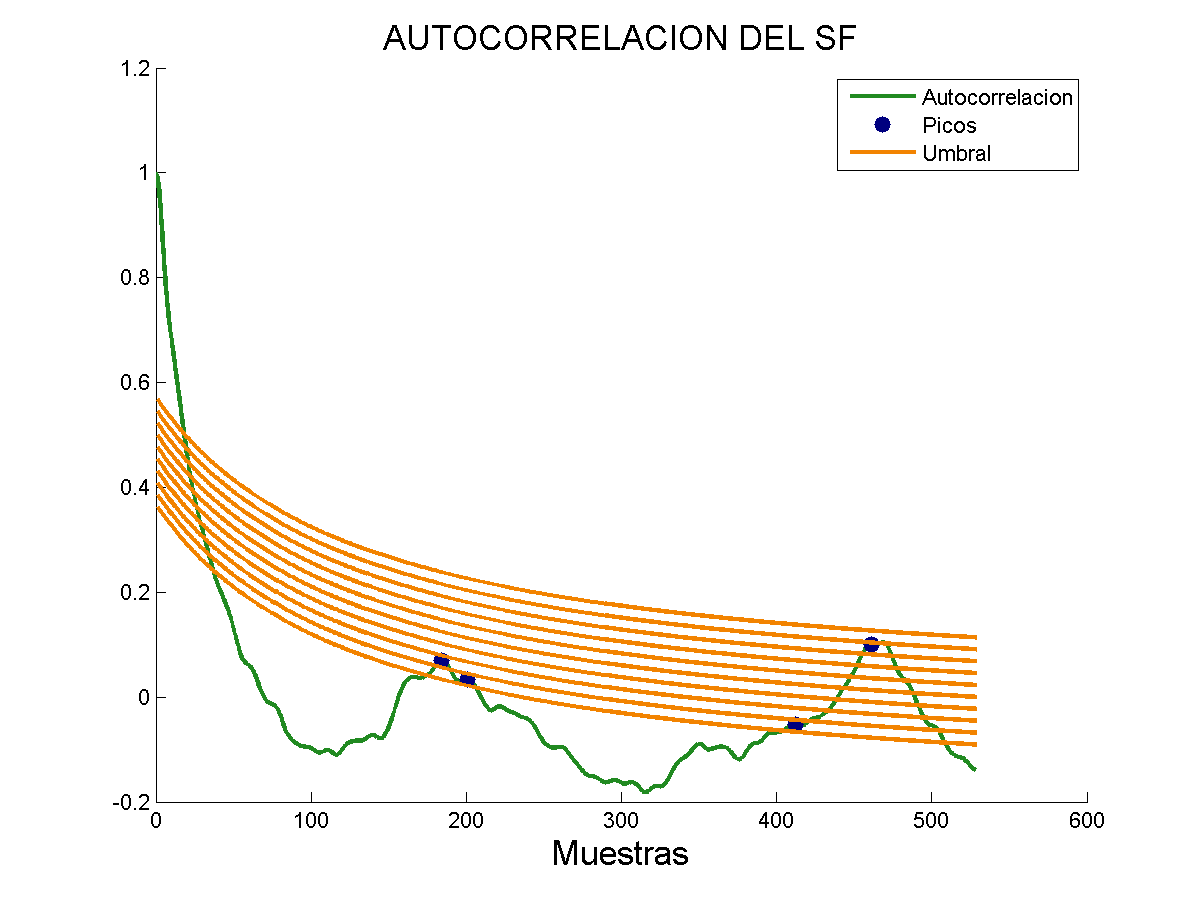
\includegraphics[width=1\textwidth]{./pics/ACF2.png}};}
\end{tikzpicture}
}


\only<7,8,9,10,11>{
\begin{tikzpicture}
\alt<11->
{\node[opacity=1]
{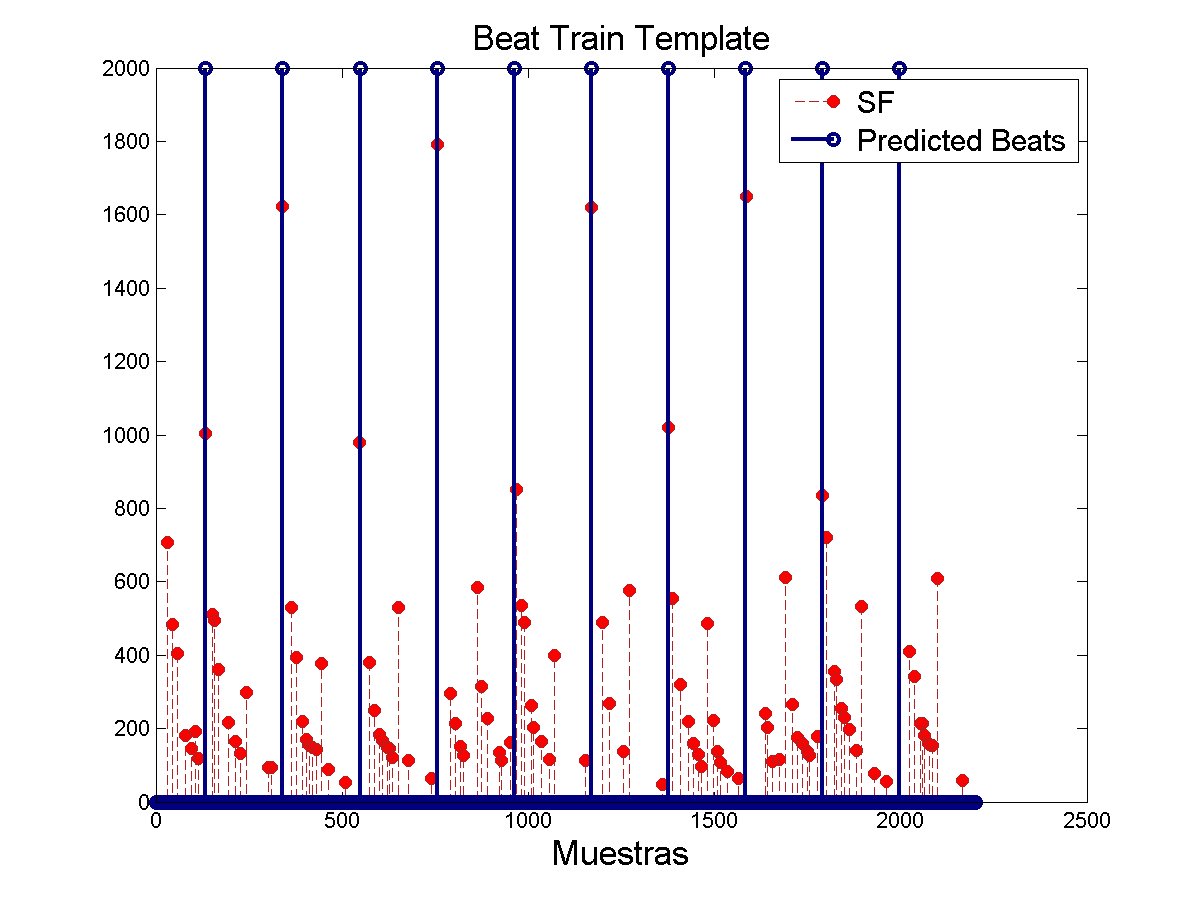
\includegraphics[width=1\textwidth]{./pics/Template.png}};}
{\node[opacity=.15]
{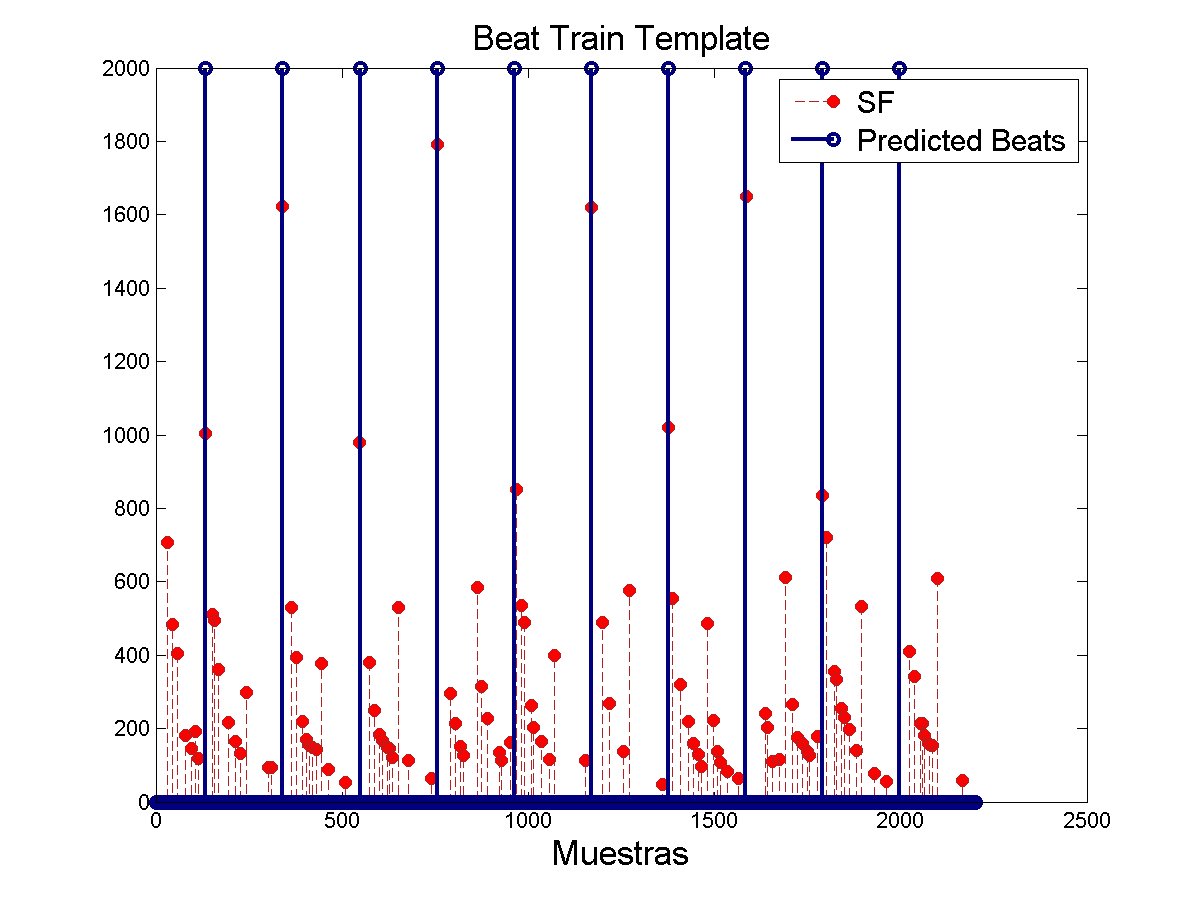
\includegraphics[width=1\textwidth]{./pics/Template.png}};}
\end{tikzpicture}
}

\only<12-16>{
\begin{tikzpicture}
\alt<16->
{\node[opacity=1]
{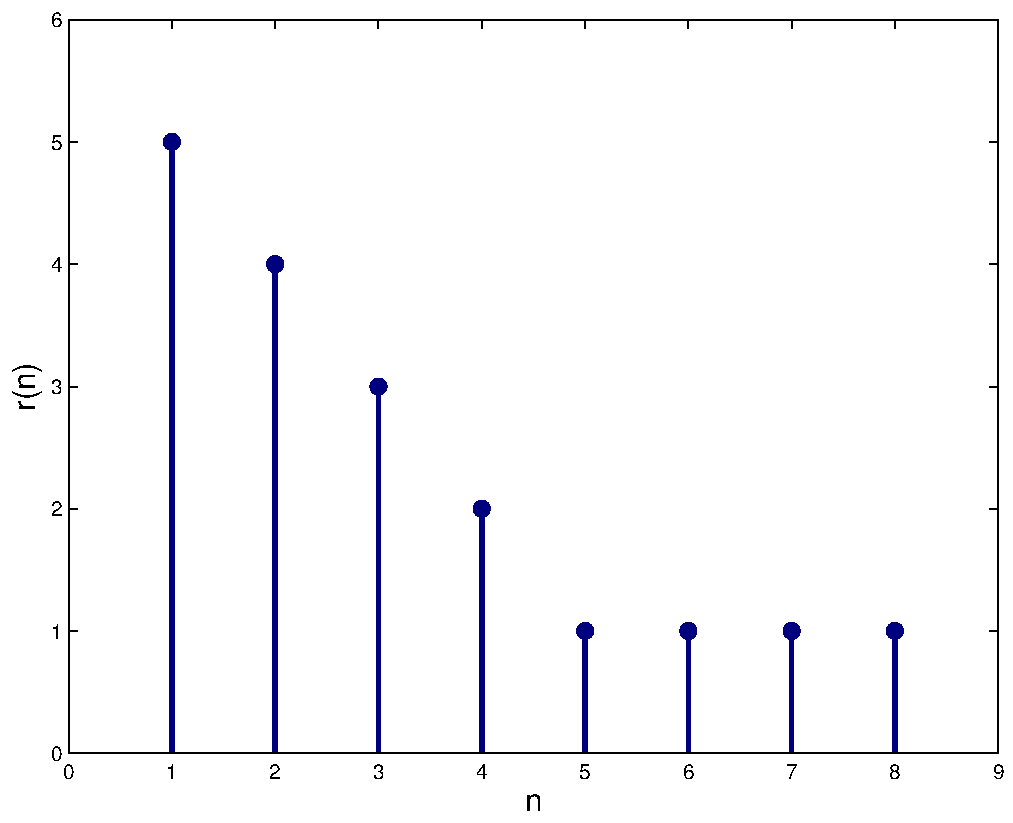
\includegraphics[width=1\textwidth]{./pics/r.pdf}};}
{\node[opacity=.15]
{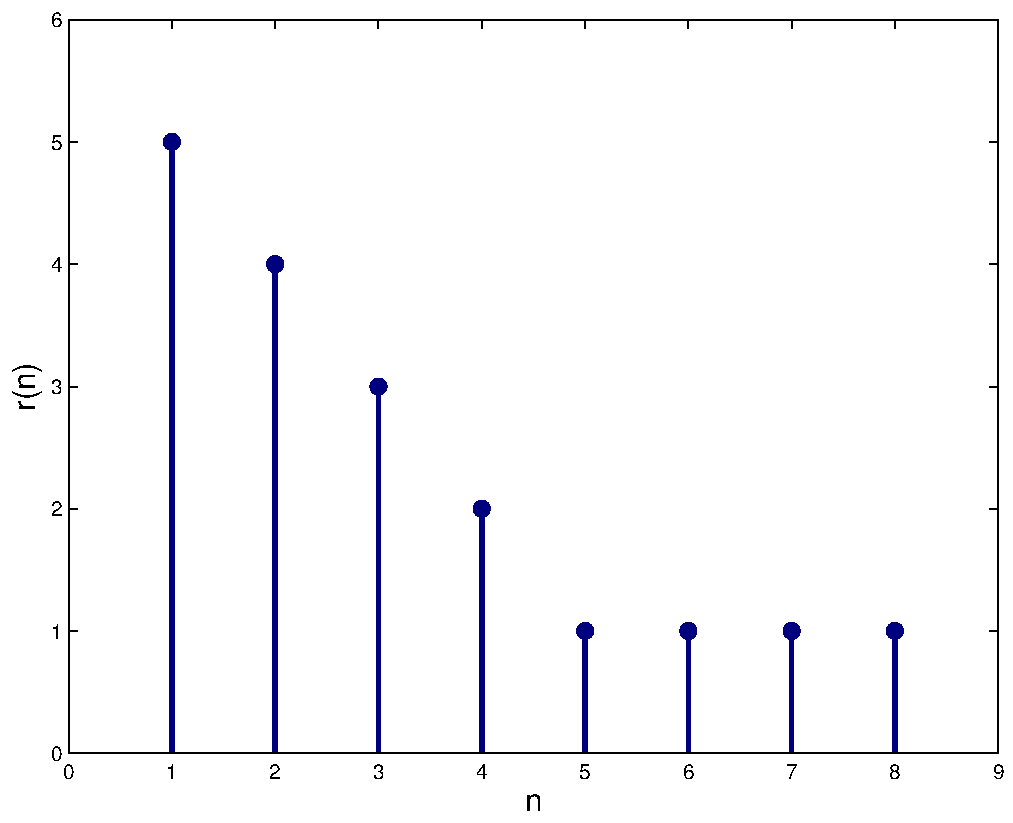
\includegraphics[width=1\textwidth]{./pics/r.pdf}};}
\end{tikzpicture}
}

\only<17 >{
\begin{tikzpicture}
\alt<17->
{\node[opacity=1]
{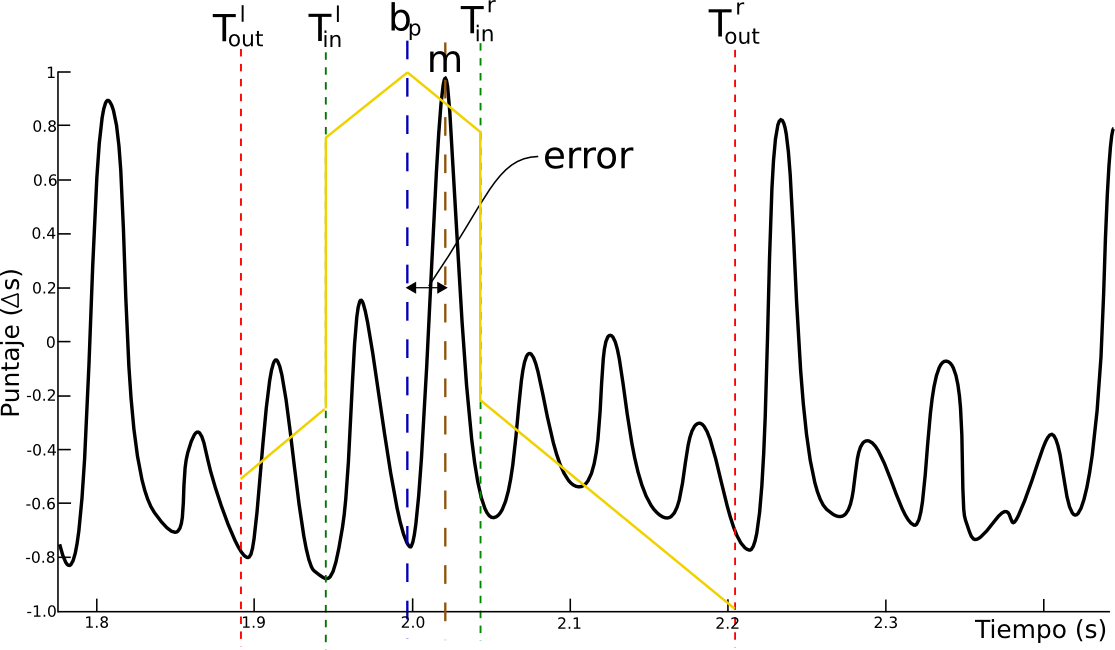
\includegraphics[width=1\textwidth]{./pics/graficamejor.png}};}
{\node[opacity=.15]
{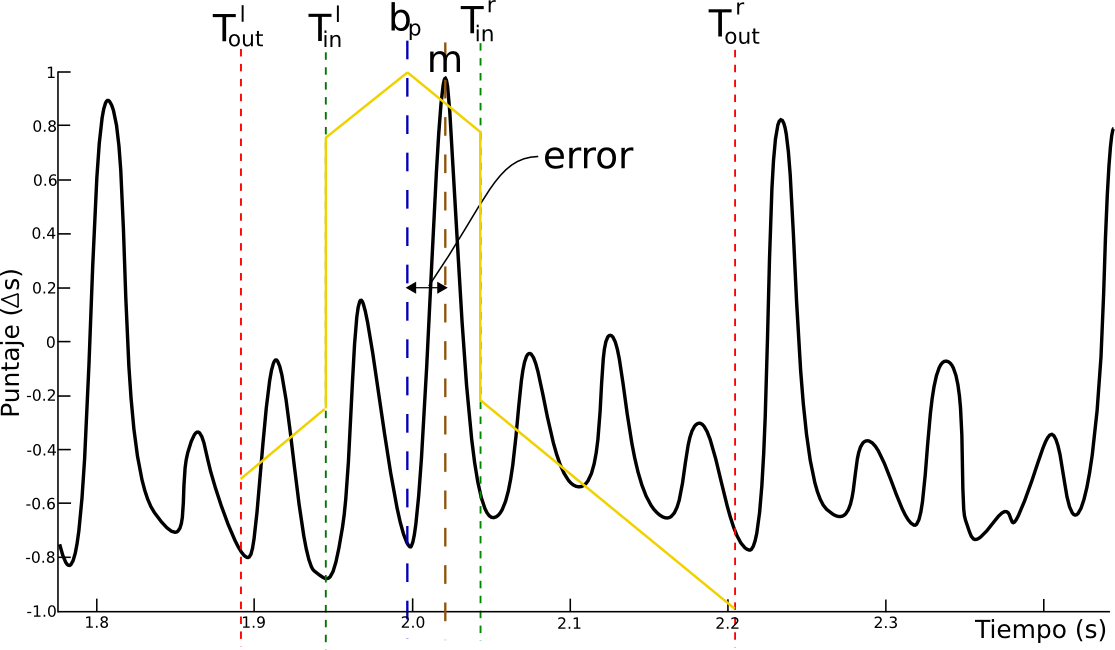
\includegraphics[width=1\textwidth]{./pics/graficamejor.png}};}
\end{tikzpicture}
}


\end{scriptsize}

\vspace*{-205pt}
\begin{block}<5>{Promedio de BPM}
El pico mas alto corresponde a 120BPM
\end{block}

\vspace*{-44pt}
\begin{block}<6>{Umbral variable}
Para garantizar la detección de picos
\end{block}

\end{columns}
%% -----------------------------------------------------------------

\end{frame}




\section{Beat-Tracking}
% ========================= FRAME ===============================
% ===============================================================
\begin{frame}
\frametitle{Beat Tracking}
%\begin{scriptsize}
%\only<2->{
%\vspace*{-10pt}
%\begin{block}{Idea}
%Supervisar flujo de entrada y mantener balance entre inercia y rapidez de la respuesta
%\end{block}
%}
%\end{scriptsize}

\only<1-4>{
\begin{scriptsize}
\vspace*{-10pt}
\begin{block}{\emph{Agent Referee}}
Evalúa la distancia entre la predicción del \emph{beat} ($b_p$) y el máximo local ($m$) de $SF$. $P_m$ es el máximo período permitido
$$\begin{cases}
\Delta s = \left(1-\frac{|error|}{T^r_{out}} \right)\frac{P_i}{P_m}SF(m), & \exists m \in T_{in}\\
\Delta s = -\left(\frac{|error|}{T^r_{out}} \right)\frac{P_i}{P_m}SF(m), & \exists m \in T_{out}\\
\end{cases}$$
\end{block}
\end{scriptsize}
}

\begin{columns}
\column{2in}

\begin{scriptsize}

\only<2-4>{
Niveles de toleracia: $T_{in}\in[T_{in}^l,T_{in}^r]$ y $T_{out}\in[T_{out}^l,T_{in}^l] \bigcup [T_{in}^r,T_{out}^r]$

\begin{figure}[h!]
  \begin{center}
  \vspace*{-10pt}
  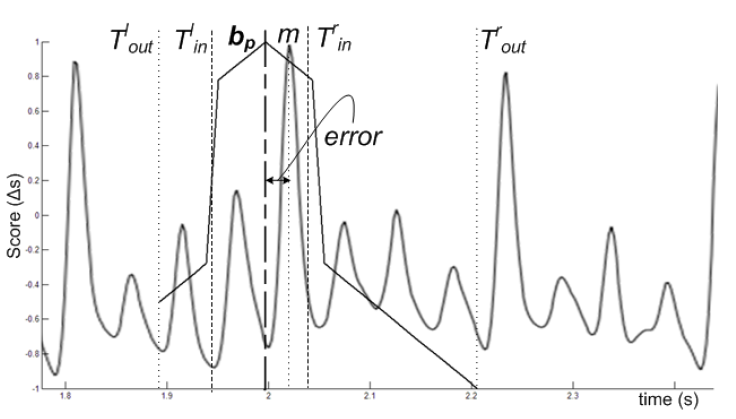
\includegraphics[width=.9\textwidth]{./pics/grafica.png}
  \end{center}
  \vspace{-10pt}
   \label{fig:grafica}
\end{figure}
}

\only<5->{
\begin{itemize} \item \textbf{Descarte de agentes} \end{itemize}
}

\only<6->{
\vspace{10pt}
\begin{description}
  \item<6->[\alert<6>{-Replacement:}]
  \vspace{10pt}
  \item<7->[\alert<7>{-Redundancy:}]
  \vspace{10pt}
  \item<8->[\alert<8>{-Obsolescence:}]
  \vspace{10pt}
  \item<9->[\alert<9>{-Loss:}]
  \vspace{10pt}
\end{description}

}


\end{scriptsize}



\column{2in}
\vspace*{-10pt}
\begin{scriptsize}

\only<3-4>{
\begin{itemize} \item \textbf{$T_{in}\in[T_{in}^l,T_{in}^r]$} \end{itemize}
$$
\begin{cases}
P_i = P_i+0.25*error\\
\phi_i = \phi_i+0.25*error
\end{cases}
$$
}
\only<4>{
\begin{itemize} \item \textbf{$T_{out}\in[T_{out}^l,T_{in}^l] \bigcup [T_{in}^r,T_{out}^r]$} \end{itemize}
El agente mantiene su período y fase y además crea 3 ``hijos'' variando dichos parámetros
}

\only<6>{
\vspace*{60pt}
\begin{block}{}
Si es el peor de un grupo de agentes que alcanzó su máximo, y su puntuación es inferior a una nueva creación de agente
\end{block}
}

\only<7>{
\vspace*{60pt}
\begin{block}{}
Para incrementar la eficiencia del algoritmo, se elimina un agente si se duplica el trabajo de un agente de score alto, si sus períodos difieren menos de 11,6ms y sus fases menos de 23,2ms
\end{block}
}

\only<8>{
\vspace*{60pt}
\begin{block}{}
Se elimina un agente si la diferencia entre su puntuación y el mejor agente es mayor que el 80\%
\end{block}
}

\only<9>{
\vspace*{60pt}
\begin{block}{}
Se descarta una agente si parece estar ``perdido'', es decir, si su predicción de beat cae 8 veces fuera de la ventana de tolerancia interior
\end{block}
}

\end{scriptsize}
\end{columns}


\end{frame}



\section{Ejemplo 1}
% ========================= FRAME ===============================
% ===============================================================
\begin{frame}
\frametitle{Ejemplos}

\only<1->{
\vspace*{10pt}
\begin{scriptsize}
\begin{itemize} \item \textbf{Caso de buen funcionamiento} \end{itemize}
\end{scriptsize}
}



\begin{columns}
\column{1.5in}

\begin{scriptsize}


\only<2>{
\vspace*{50pt}
\begin{block}{Pre-Tracking}
El valor del mayor pico corresponde a xxBPM
\end{block}
}

\only<3>{
\vspace*{50pt}
\begin{block}{Beat Tracking}
El 1er agente es el ganador para esta pieza
\end{block}
}

\only<4>{
\vspace*{50pt}
\begin{block}{Agente 1}
\begin{center}
\movie[label=cells]{}{./music/datos2_2_A_tracked.wav}
\hyperlinkmovie[]{cells}{\beamergotobutton{PLAY}}
\end{center}
\end{block}
}






\end{scriptsize}


\column{3in}
\begin{scriptsize}


\only<1-2 >{
\begin{tikzpicture}
\alt<2>
{\node[opacity=1]
{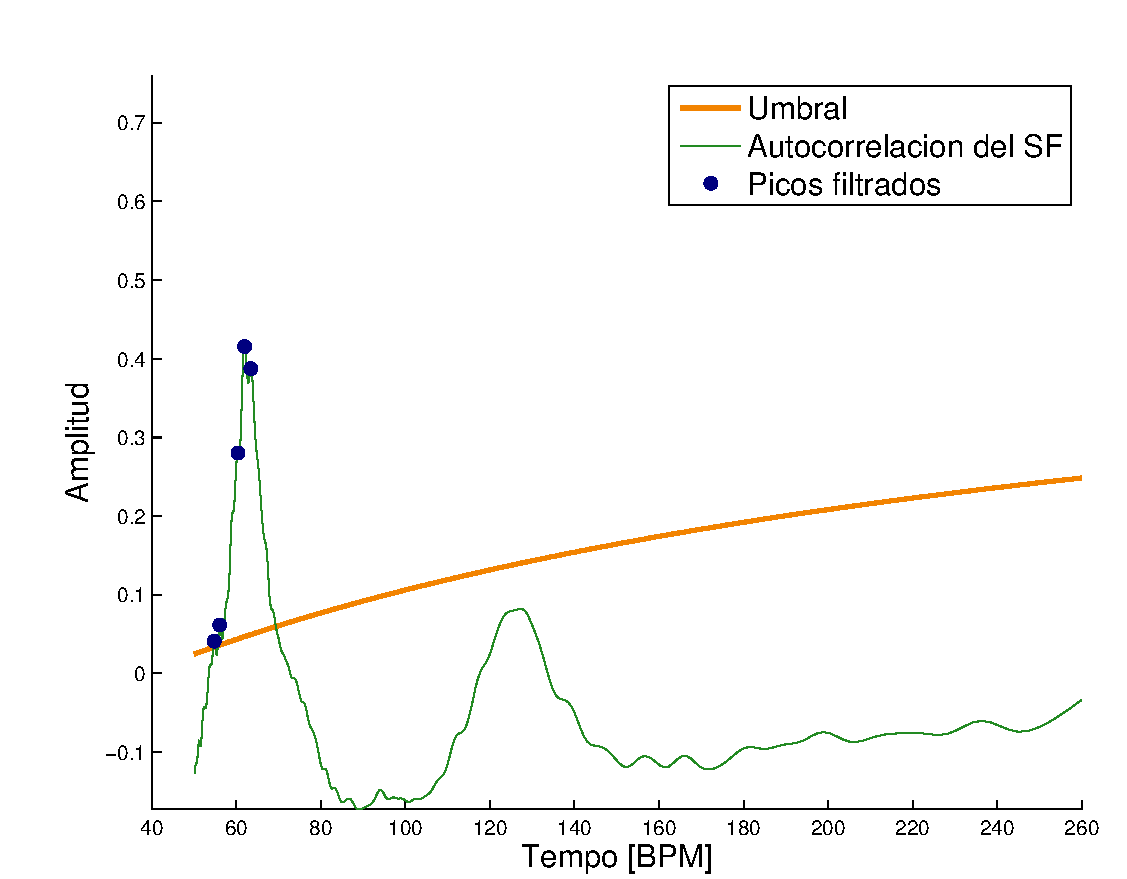
\includegraphics[width=1\textwidth]{./pics/datos_2_2_A_autocorr.pdf}};}
{\node[opacity=.15]
{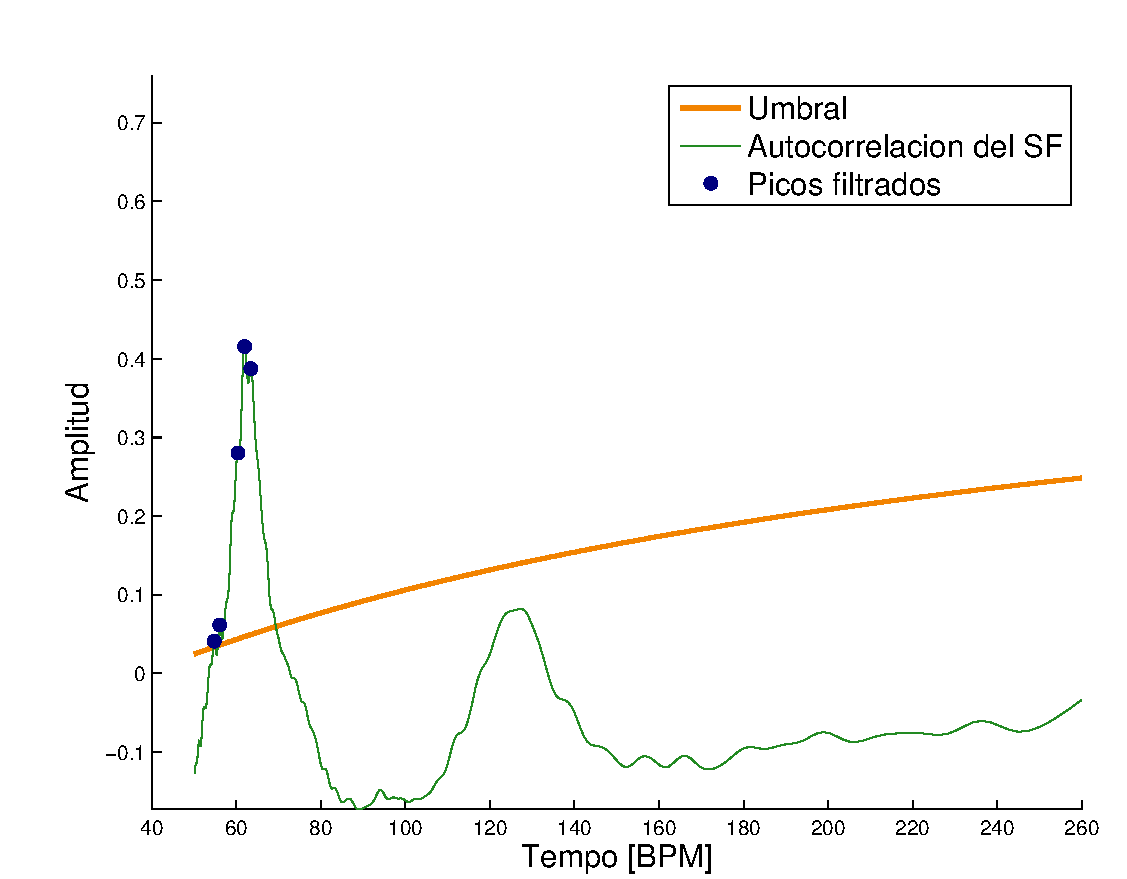
\includegraphics[width=1\textwidth]{./pics/datos_2_2_A_autocorr.pdf}};}
\end{tikzpicture}
}

\only<3>{
\begin{tikzpicture}
\alt<3>
{\node[opacity=1]
{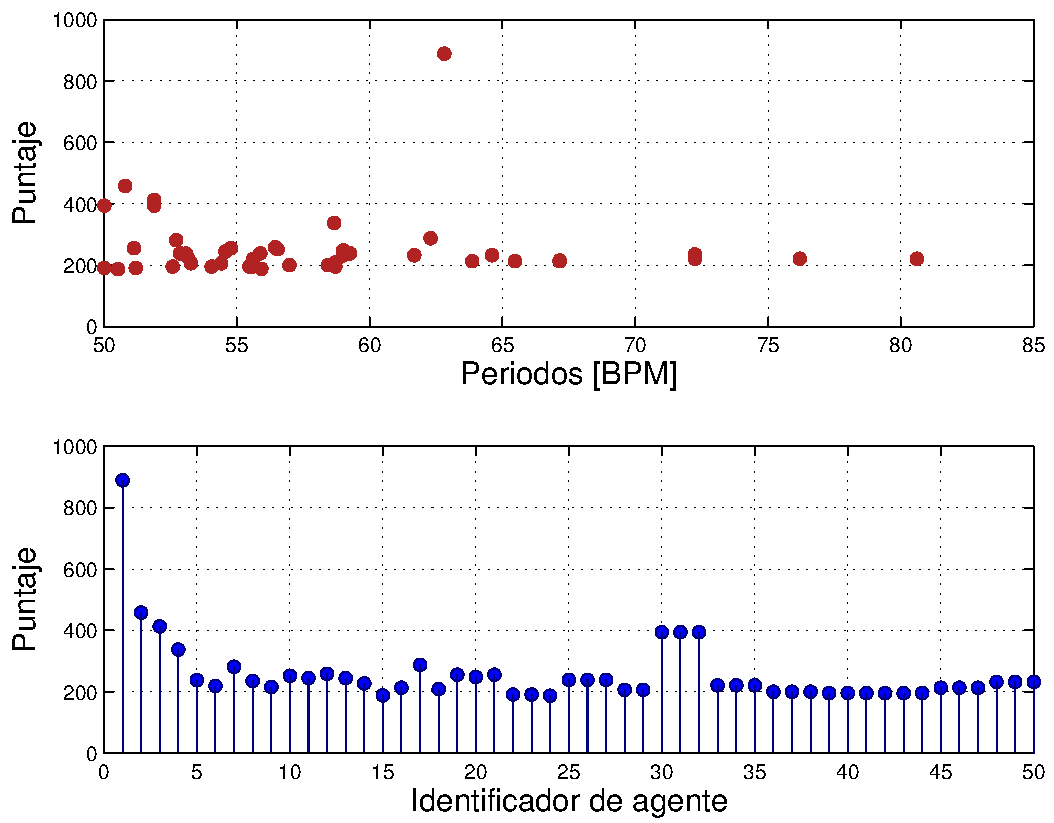
\includegraphics[width=1\textwidth]{./pics/datos_2_2_A_agents.pdf}};}
{\node[opacity=.15]
{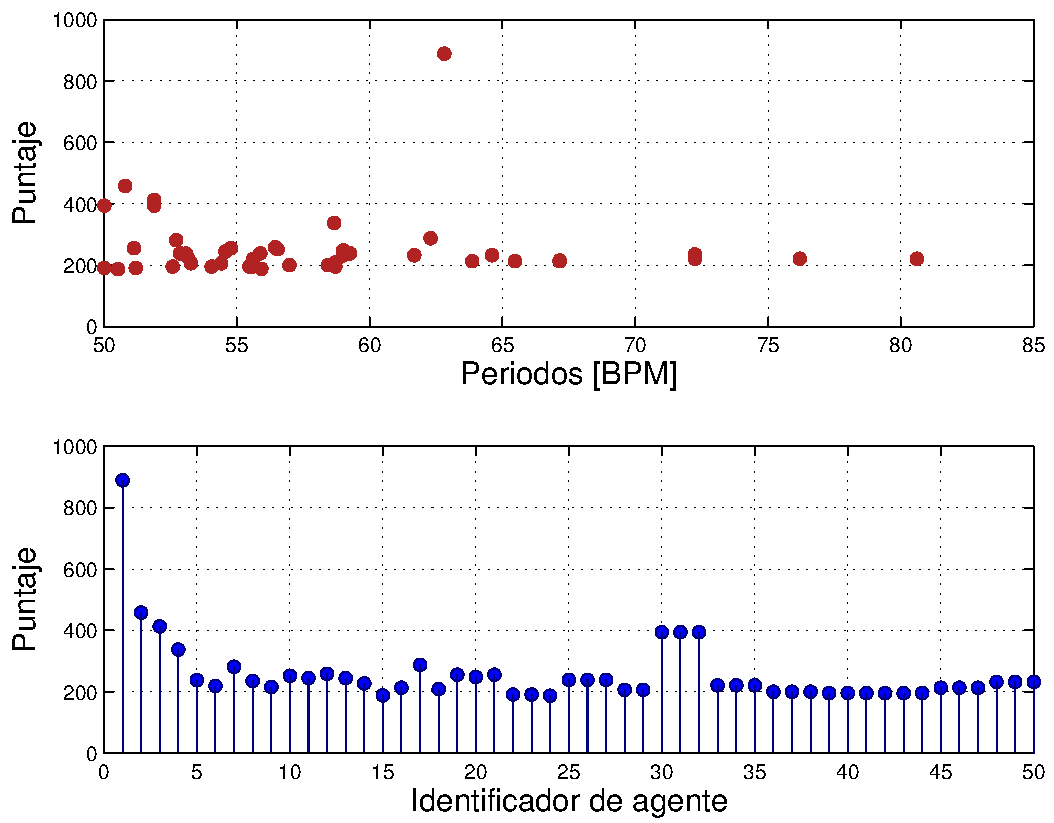
\includegraphics[width=1\textwidth]{./pics/datos_2_2_A_agents.pdf}};}
\end{tikzpicture}
}

\only<4>{
\begin{tikzpicture}
\alt<4>
{\node[opacity=1]
{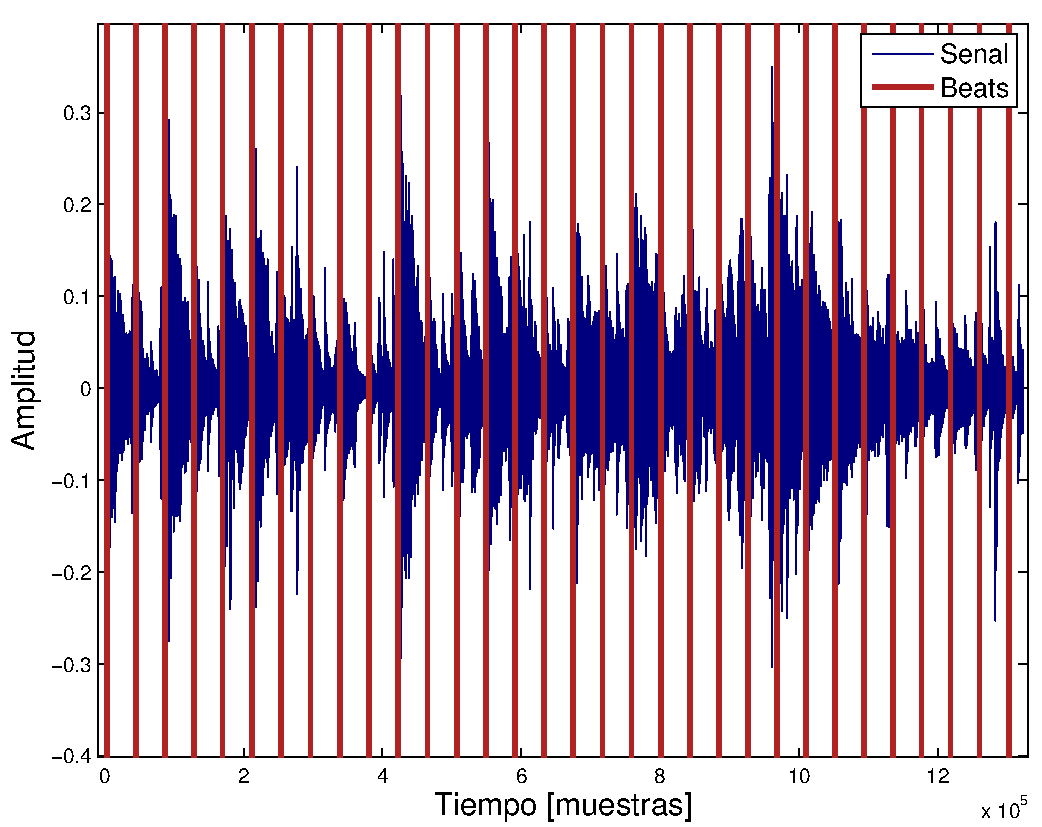
\includegraphics[width=1\textwidth]{./pics/datos_2_2_A_beats_bien.pdf}};}
{\node[opacity=.15]
{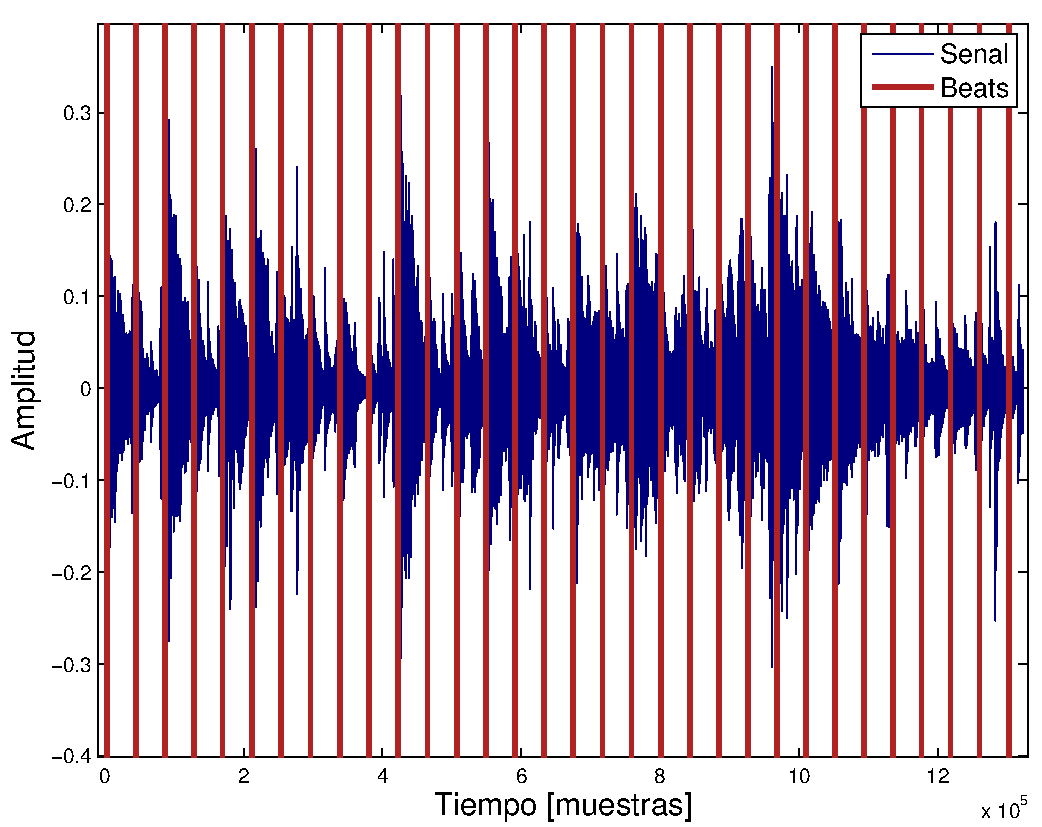
\includegraphics[width=1\textwidth]{./pics/datos_2_2_A_beats_bien.pdf}};}
\end{tikzpicture}
}

\end{scriptsize}
\end{columns}

\only<5>{
\vspace*{50pt}
\begin{scriptsize}
\begin{block}{Agente 1}
\begin{center}
\rowcolors{1}{RoyalBlue!5}{RoyalBlue!20}
\begin{tabular}{rllll} \hline
Cont-Based: & cC: 100.00 & cT: 100.00 & aC:100.00 & aT:100.00 \\ \hline
F-Mesure: & f: 94.44 & p: 94.44 & r: 94.44 & a: 89.47 \\ \hline
\end{tabular}
\end{center}
\end{block}
\end{scriptsize}
}


\end{frame}



\section{Ejemplo 2}
% ========================= FRAME ===============================
% ===============================================================
\begin{frame}
\frametitle{Ejemplos}

\only<1->{
\vspace*{10pt}
\begin{scriptsize}
\begin{itemize} \item \textbf{Caso de funcionamiento comprometido} \end{itemize}
\end{scriptsize}
}



\begin{columns}
\column{1.5in}

\begin{scriptsize}


\only<2>{
\vspace*{50pt}
\begin{block}{Pre-Tracking}
El valor del mayor pico corresponde a xxBPM
\end{block}
}

\only<3>{
\vspace*{50pt}
\begin{block}{Beat Tracking}
El 2do agente es el ganador para esta pieza
\end{block}
}

\only<4>{
\vspace{50pt}
\begin{block}{Agente 2}
\begin{center}
\movie[label=cells2]{}{./music/datos2_14_A_tracked.wav}
\hyperlinkmovie[]{cells2}{\beamergotobutton{PLAY}}
\end{center}
\end{block}
}

\only<5>{
\vspace*{50pt}
\begin{block}{Agente 1}
\begin{center}
\movie[label=cells2]{}{./music/datos2_14_A_tracked.wav}
\hyperlinkmovie[]{cells2}{\beamergotobutton{PLAY}}
\end{center}
\end{block}
}




\end{scriptsize}


\column{3in}
\begin{scriptsize}


\only<1-2 >{
\begin{tikzpicture}
\alt<2>
{\node[opacity=1]
{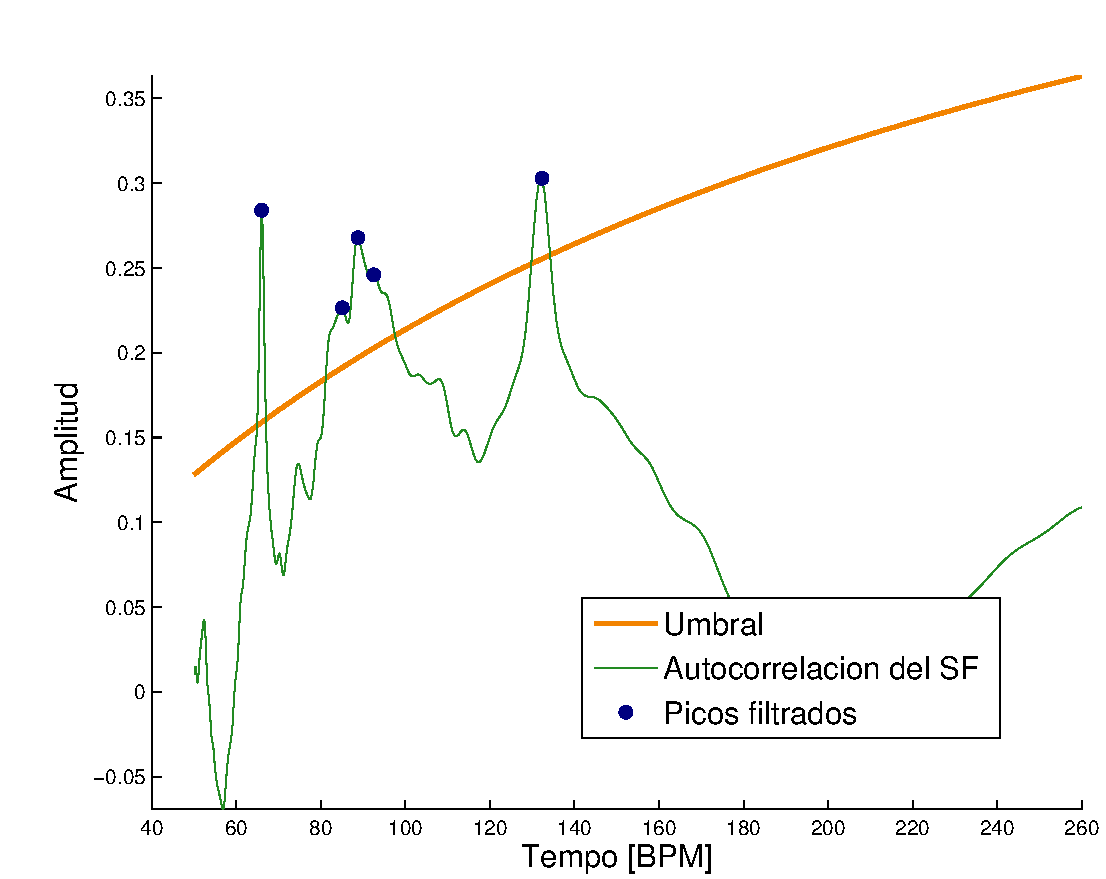
\includegraphics[width=1\textwidth]{./pics/datos_2_14_A_autocorr2.pdf}};}
{\node[opacity=.15]
{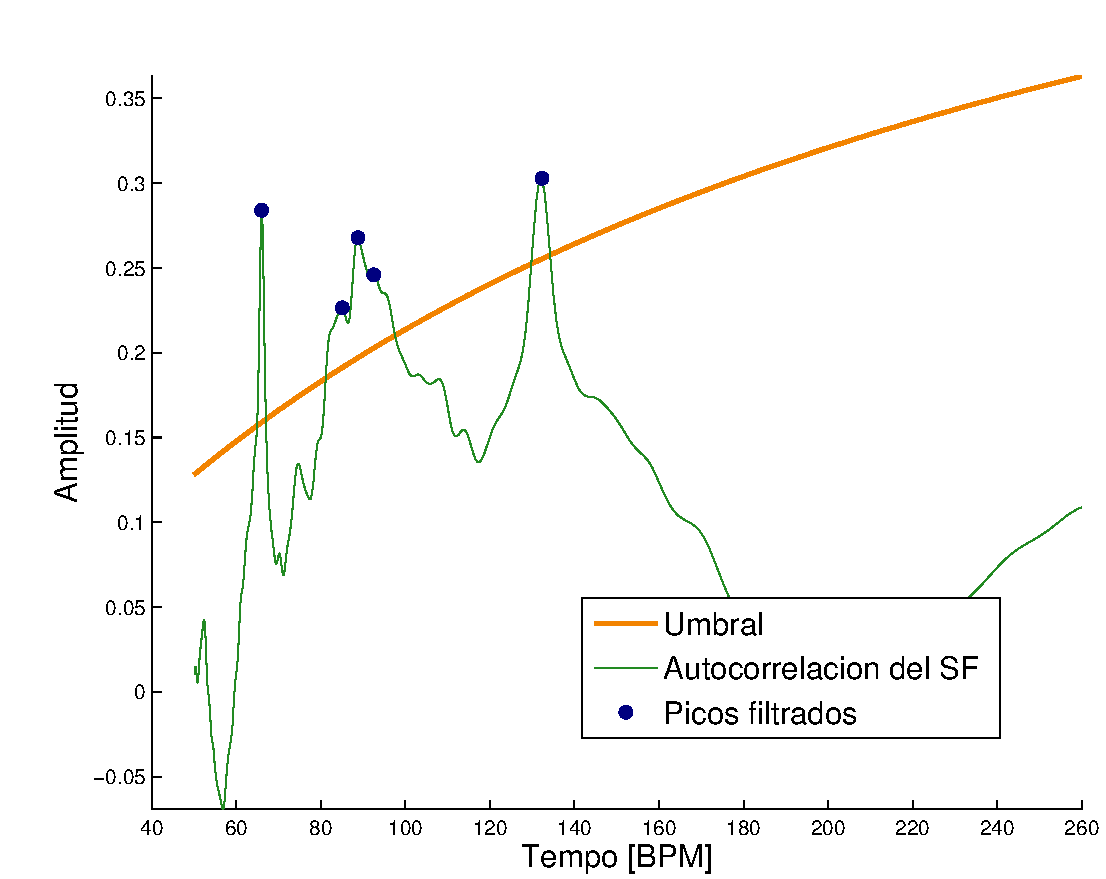
\includegraphics[width=1\textwidth]{./pics/datos_2_14_A_autocorr2.pdf}};}
\end{tikzpicture}
}

\only<3>{
\begin{tikzpicture}
\alt<3>
{\node[opacity=1]
{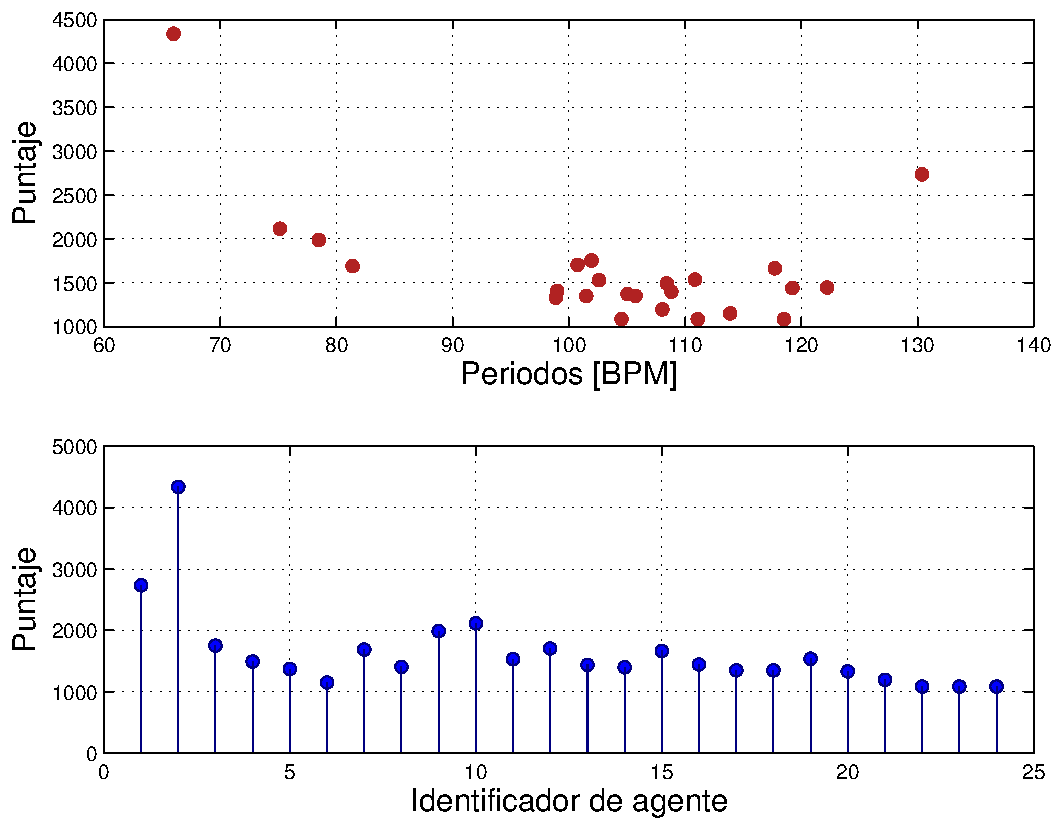
\includegraphics[width=1\textwidth]{./pics/datos_2_14_A_agents.pdf}};}
{\node[opacity=.15]
{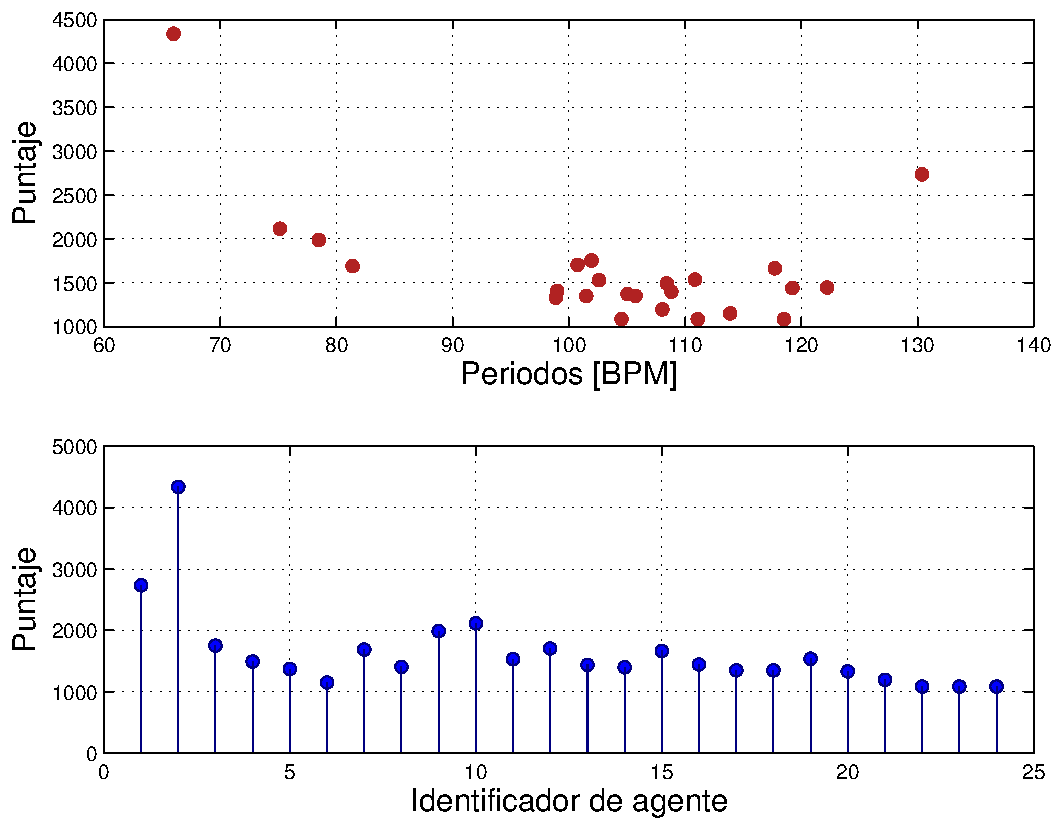
\includegraphics[width=1\textwidth]{./pics/datos_2_14_A_agents.pdf}};}
\end{tikzpicture}
}

\only<4>{
\begin{tikzpicture}
\alt<4>
{\node[opacity=1]
{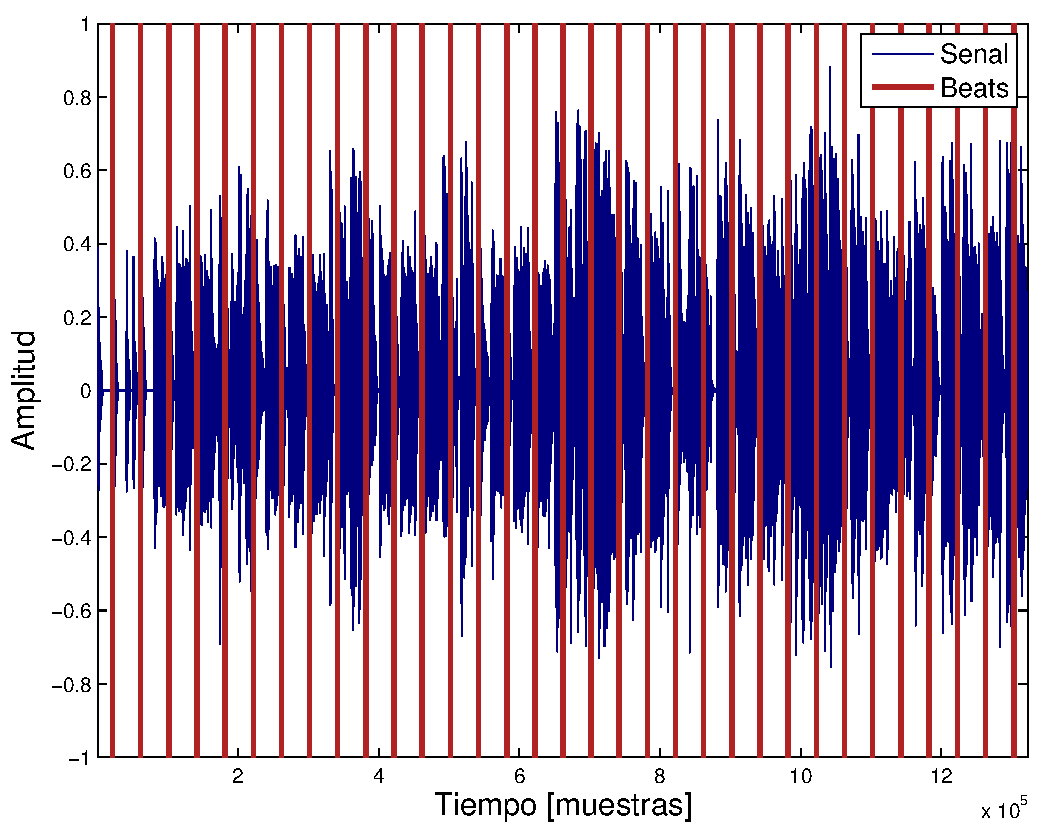
\includegraphics[width=1\textwidth]{./pics/datos_2_14_A_beats_lento.pdf}};}
{\node[opacity=.15]
{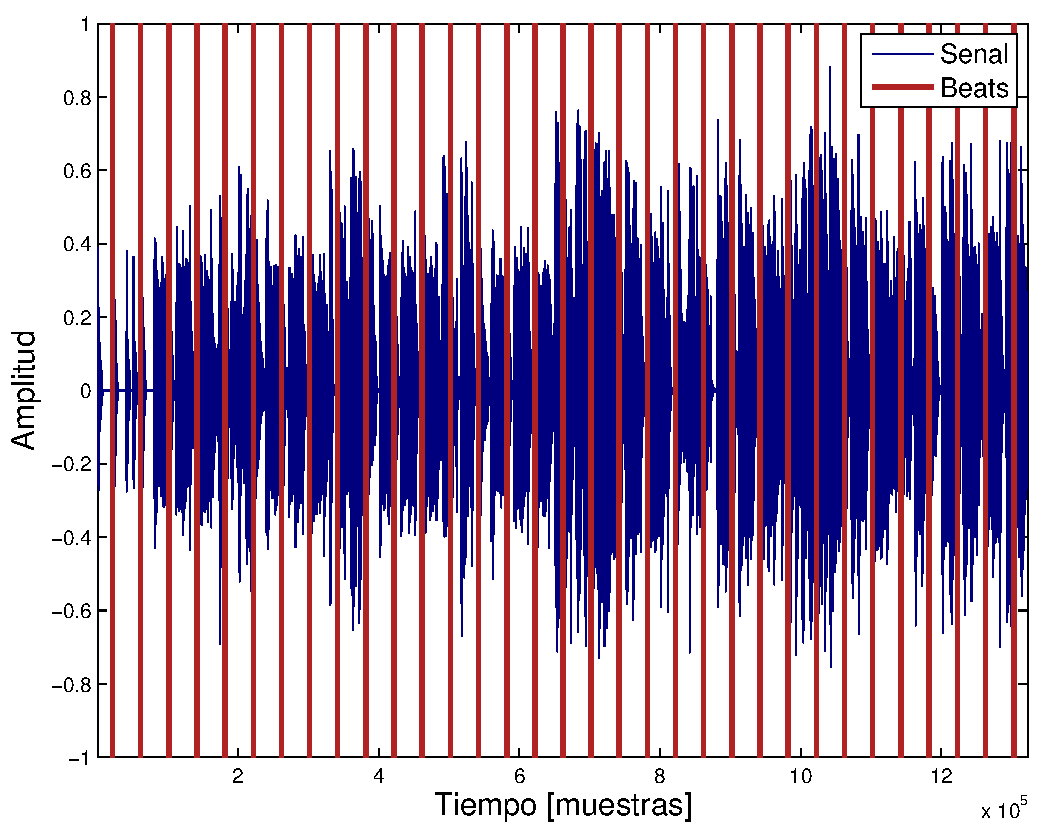
\includegraphics[width=1\textwidth]{./pics/datos_2_14_A_beats_lento.pdf}};}
\end{tikzpicture}
}

\only<5>{
\begin{tikzpicture}
\alt<5>
{\node[opacity=1]
{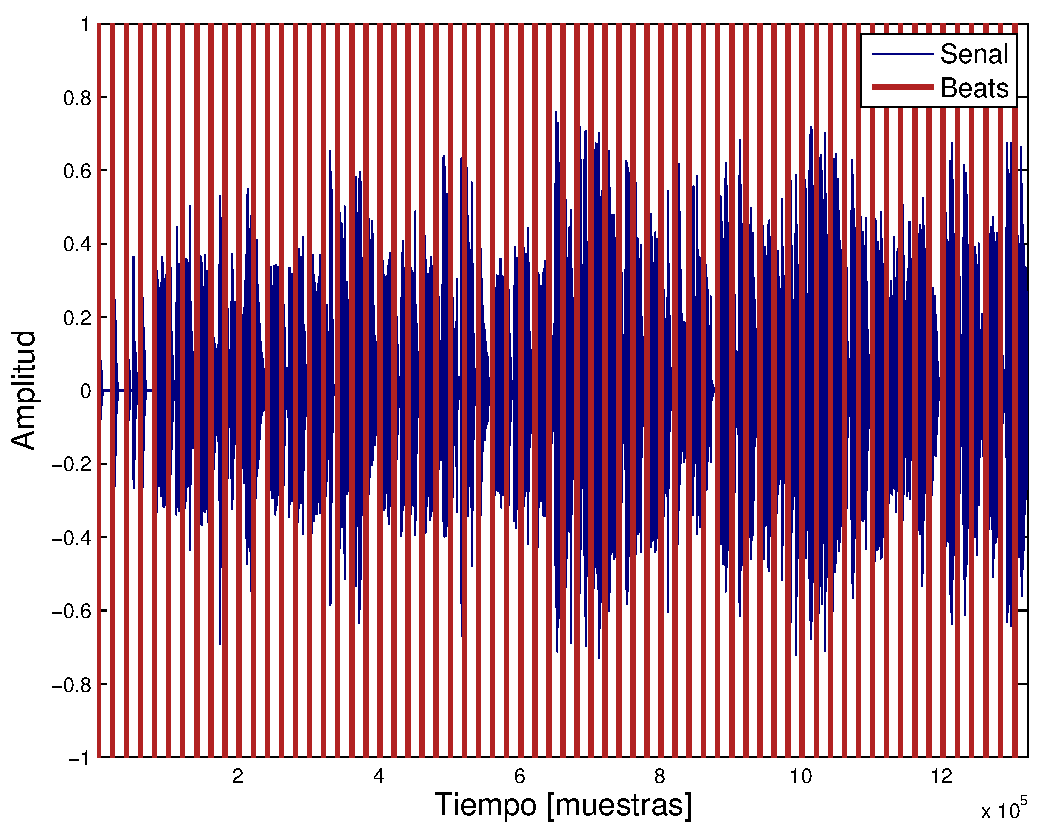
\includegraphics[width=1\textwidth]{./pics/datos_2_14_A_beats_bien.pdf}};}
{\node[opacity=.15]
{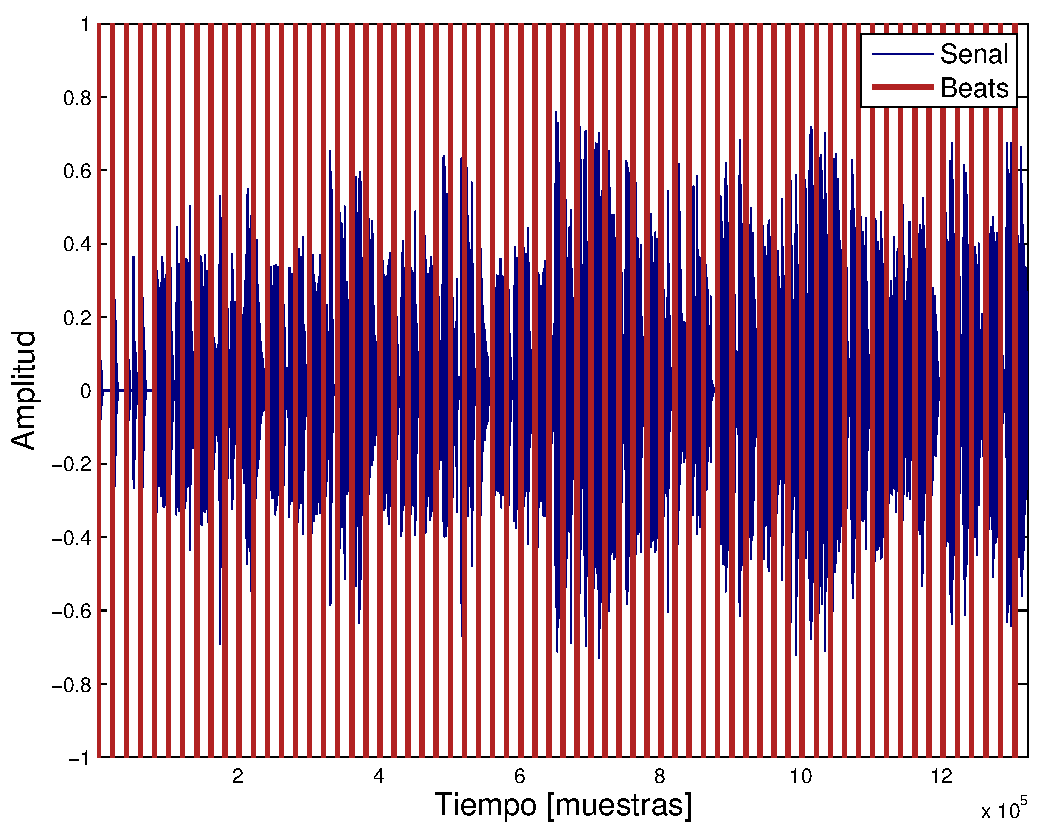
\includegraphics[width=1\textwidth]{./pics/datos_2_14_A_beats_bien.pdf}};}
\end{tikzpicture}
}


\end{scriptsize}
\end{columns}

\only<6->{
\vspace*{20pt}
\begin{scriptsize}
\begin{block}{Agente 2}
\begin{center}
\rowcolors{1}{RoyalBlue!5}{RoyalBlue!20}
\begin{tabular}{rllll} \hline
Cont-Based: & cC: 00.00 & cT: 00.00 & aC: 100.00 & aT: 100.00 \\ \hline
F-Mesure: & f: 67.47 & p: 100.00 & r: 50.91 & a: 50.91 \\ \hline
\end{tabular}
\end{center}
\end{block}
\end{scriptsize}
}

\only<7->{
\vspace*{10pt}
\begin{scriptsize}
\begin{block}{Agente 1}
\begin{center}
\rowcolors{1}{RoyalBlue!5}{RoyalBlue!20}
\begin{tabular}{rllll} \hline
Cont-Based: & cC: 100.00 & cT: 100.00 & aC: 100.00 & aT: 100.00 \\ \hline
F-Mesure: & f: 100.00 & p: 100.00 & r: 100.00 & a: 100.00 \\ \hline
\end{tabular}
\end{center}
\end{block}

\end{scriptsize}
}


\end{frame}

\section{Conclusiones}
% ========================= FRAME ===============================
% ===============================================================
\begin{frame}
\frametitle{Conlusiones}
\begin{scriptsize}
\vspace*{30pt}
\begin{itemize}
  \item<1-> \alert<1>{Desempeño aceptable} 
  \vspace*{10pt}
  \item<2-> \alert<2>{Dudas de implementación}
  \vspace*{10pt}
  \item<3-> \alert<3>{Se puede mejorar la elección del agente ganador}
  \vspace*{10pt}
  \item<4-> \alert<4>{Tiene robustez}
  \vspace*{10pt}
  \item<5-> \alert<5>{Buena relación entre inercia y rapidez de respuesta}
  \vspace*{10pt}
  \item<6-> \alert<6>{Buenos resultados ``auditivos''}
\end{itemize}


\end{scriptsize}

\end{frame}

\section{Referencias}
% ===============================================================
% ========================= FRAME ===============================
% ===============================================================
\begin{frame}
\frametitle{Referencias:}
\begin{thebibliography}{99}
\begin{small}

\bibitem{bib:algo}Jo\~ao Lobato Oliveira, Fabien Gouyon, Luis Gustavo Martins, Luis Paulo Reis, IBT: A real time tempo and beat tracking system, In \emph{11th International Society for Music Information Retrieval Conference, ISMIR}, 2010.

\bibitem{bib:asdf}S. Dixon. Automatic extraction of tempo and beat from
expressive performances. In \emph{Journal of New Music Research, 30(1):39–58}, 2001.

\bibitem{bib:otra_cosa}S. Dixon. Onset detection revisited. In \emph{in Proceedings of the 9th International Conference on Digital Audio Effects}, pages 133–13, Montreal, Canada, 2006.

\bibitem{bib:y_asi}F. Gouyon, P. Herrera, and P. Cano. Pulse-dependent analyses of percussive music. In \emph{AES 22nd International Conference on Virtual}, Synthetic and Entertainment Audio, 2002.

\end{small}
\end{thebibliography}
\end{frame}







\end{document}





% ========================= FRAME ===============================
% ===============================================================
\begin{frame}
\frametitle{Title}
\begin{columns}
\column{2in}
\vspace*{-15pt}
\begin{scriptsize}


\begin{block}{title of the bloc}
bloc text
\end{block}
\begin{exampleblock}{title of the bloc}
bloc text
\end{exampleblock}
\begin{alertblock}{title of the bloc}
bloc text
\end{alertblock}


\end{scriptsize}
\column{2in}
\begin{scriptsize}

\begin{itemize}
	\item \textbf{Item 1}:\pause
  	\begin{itemize*}
	  \item subitem 1 \pause
	  \item subitem 2 \pause
	  \item subitem 3 \pause
	\end{itemize*}
	\item \textbf{Item 2}
\end{itemize}

\end{scriptsize}
\end{columns}
\end{frame}



% ================ FRAME TPICO CON FIGURA ======================
% ===============================================================

\begin{frame}
\frametitle{Qu es un Parcial?}

\begin{columns}

\column{2in}
\vspace{-25pt}
\begin{figure}[h!]
  \begin{center}
  \includegraphics[width=.85\textwidth]{./Pics/Espectrograma_ejemplo.jpg}
  \end{center}
  \vspace{-10pt}
  \caption{Espectrograma}
  \label{fig:espectrograma_ejemplo}
\end{figure}

\column{2in}
\begin{itemize}
	\item \textbf{Item 1}:\pause
  	\begin{itemize*}
	  \item subitem 1 \pause
	  \item subitem 2 \pause
	  \item subitem 3 \pause
	\end{itemize*}
	\item \textbf{Item 2}
\end{itemize}

\end{columns}
\end{frame}




% ======================== FIGURAS ==============================
% ===============================================================

\begin{figure}[h!]
	\centering
	\includegraphics[width=0.75\textwidth]{./Pics/		.eps}
	\caption{		}
	\label{fig:		}
\end{figure}

\begin{figure} [h!]
  \centering
  \subfloat[caption 1]{\label{fig:		}
  		\includegraphics[width=0.45\textwidth]
  			{./Pics/		.eps}}
  \subfloat[caption 2]{\label{fig:		}
  		\includegraphics[width=0.45\textwidth]
  			{./Pics/ 		.eps}}
  \caption{Caption general}
  \label{fig:	label general	}
\end{figure}

\begin{wrapfigure}{l}{0.6\textwidth}
  \vspace{-20pt}
  \begin{center}
    \includegraphics[width=0.45\textwidth]
    	{./Pics/		.eps}
  \end{center}
  \vspace{-20pt}
  \caption{		}
  \label{ 		}
  \vspace{-10pt}
\end{wrapfigure}

\begin{figure} [h!]
  \begin{center}
    \begin{tabular}{cc}
      \resizebox{50mm}{!}
      	{\includegraphics{./Pics/ 	.eps}} &
      \resizebox{50mm}{!}
      	{\includegraphics{./Pics/	.eps}} \\
      \resizebox{50mm}{!}
      	{\includegraphics{./Pics/	.eps}} &
      \resizebox{50mm}{!}
      	{\includegraphics{./Pics/	.eps}} \\
    \end{tabular}
    \caption{ 		}
    \label{ 		}
  \end{center}
\end{figure}
